%----------------------------------------------------------------------------------------
%	PACKAGES AND OTHER DOCUMENT CONFIGURATIONS
%----------------------------------------------------------------------------------------

\documentclass[12pt]{article}
\usepackage[utf8]{inputenc}
\usepackage[british,UKenglish,USenglish,english,american]{babel}
\usepackage{graphicx}
\usepackage{listings}
\usepackage[T1]{fontenc}
\begin{document}


\newcommand{\HRule}{\rule{\linewidth}{0.5mm}} % Defines a new command for the horizontal lines, change thickness here

\center % Center everything on the page
 
%----------------------------------------------------------------------------------------
%	HEADING SECTIONS
%----------------------------------------------------------------------------------------

\textsc{\LARGE university Jean-Jaur\`{e}s}\\[1.5cm] % Name of your university/college
\textsc{\large Projet Réseau }\\[0.5cm] % Minor heading such as course title


%----------------------------------------------------------------------------------------
%	TITLE SECTION
%----------------------------------------------------------------------------------------

\HRule \\[0.4cm]
{ \huge \bfseries DNC SERVER \\ START MANUAL}\\[0.4cm] % Title of your document
\HRule \\[1.5cm]
 %----------------------------------------------------------------------------------------
%	LOGO SECTION
%----------------------------------------------------------------------------------------


\includegraphics[scale=0.25]{logo.png}\\[1cm] % Include a department/university logo - this will require the graphicx package
 
%----------------------------------------------------------------------------------------

%----------------------------------------------------------------------------------------
%	AUTHOR SECTION
%----------------------------------------------------------------------------------------

\begin{minipage}{0.4\textwidth}
\begin{flushleft} \large
\emph{Authors:}\\
Quentin \textsc{Rouland}\\
Renan \textsc{Husson}
\end{flushleft}
\end{minipage}
~
\begin{minipage}{0.4\textwidth}
\begin{flushright} \large
\emph{To the attention of :} \\
 M.  \textsc{Jacoboni }
\end{flushright}
\end{minipage}\\[4cm]

% If you don't want a supervisor, uncomment the two lines below and remove the section above
%\Large \emph{Author:}\\
%John \textsc{Smith}\\[3cm] % Your name

%----------------------------------------------------------------------------------------
%	DATE SECTION
%----------------------------------------------------------------------------------------

{\large \today}\\[3cm] % Date, change the \today to a set date if you want to be precise




\clearpage
\tableofcontents
\clearpage
\begin{flushleft}
\section{Server}
    \subsection{Reqirement}
    You need to install python 3.4 for launch the DNC server.
    
	\subsection{Configuration}
	Before running the server, it is possible to change the default configuration file through dncServer.conf. In this file you can configure the port use and the log directory by ther server.
	
	\begin{center}
		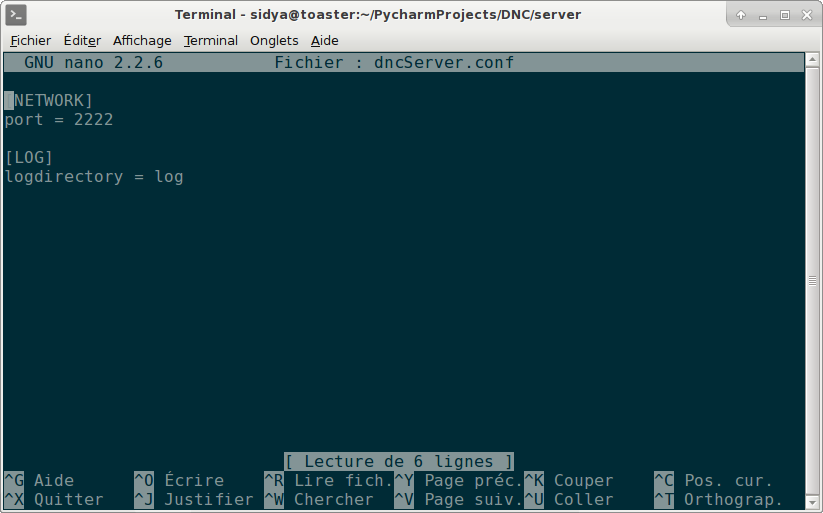
\includegraphics[scale=0.5]{config.png}
	\end{center}
	\newpage
	\subsection{Start Server}
	Just start the server with the following command :
	\begin{lstlisting}
 		python startServer.py

 	\end{lstlisting} 
 	\begin{center}
 		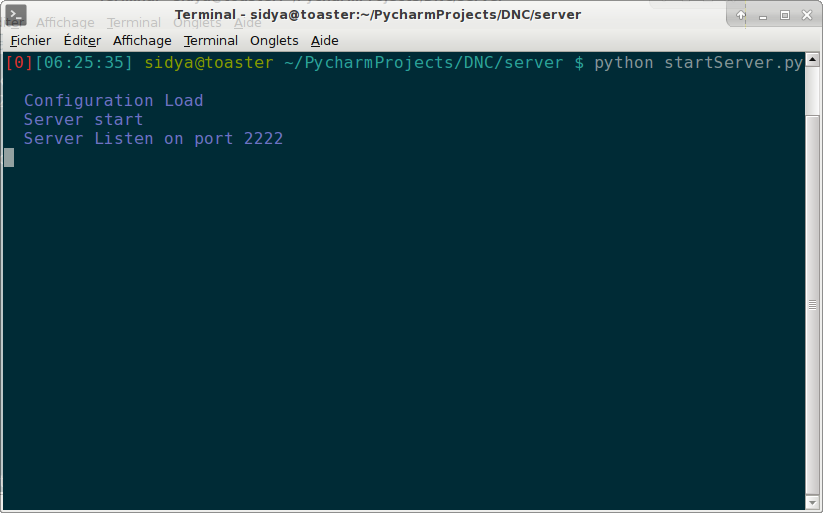
\includegraphics[scale=0.5]{start.png}
 	\end{center}
 	
 	
  

		
\end{flushleft}
\end{document}